\documentclass[11pt,compress]{beamer}
% deactivate beamer navigation
%\setbeamertemplate{navigation symbols}{}
%\usepackage{geometry}
%\geometry{papersize={180mm, 135mm}, top=-1.5mm} % 210mm, 297mm
\usepackage{../style/lmu-lecture}
\setbeamertemplate{frametitle}{\expandafter\uppercase\expandafter\insertframetitle}
%\useoutertheme{metropolis}
% remove section slides
\AtBeginSection[]
{
  \begin{frame}<beamer>
    \frametitle{Introduction to Machine Learning}
    \tableofcontents[currentsection]
  \end{frame}
}
% includepdf slides, pagecommad will set counter for framenumber
\usepackage{pdfpages}
\includepdfset{trim=0mm 0mm 0mm 0mm, pagecommand={\global\setcounter{framenumber}{\value{page}}}}
% trim=0mm 6mm 0mm 0mm, offset=0 15,
% add footer:
\usepackage{framed, color}
\usepackage{xcolor}
%\iffalse
\setbeamertemplate{footline}[text line]{%
    \noindent\hspace*{\dimexpr-\oddsidemargin-1in\relax}%
     \colorbox{white}{
     \makebox[\dimexpr\paperwidth-2\fboxsep\relax]{
     \color{black}
     \begin{minipage}[c][4.5ex][c]{0.5\linewidth}
       \secname
     \end{minipage}
     \hfill\begin{minipage}[c][4.5ex][c]{0.5\linewidth}
       \flushright
       \insertframenumber{}~/~\inserttotalframenumber~~
     \end{minipage}
     }}%
  \hspace*{-\paperwidth}
}
%\fi

\begin{document}
\setbeamercolor{background canvas}{bg=}

% General remark: hyperlinks in included pdfs are not clickable anymore in the combined pd
\section{Nested Resampling}
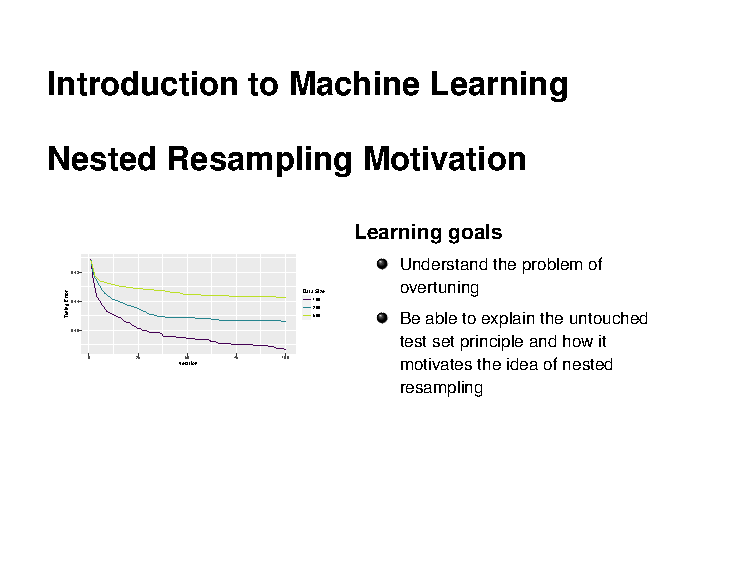
\includepdf[pages={1-last}]{slides-nested-nestedintro.pdf}
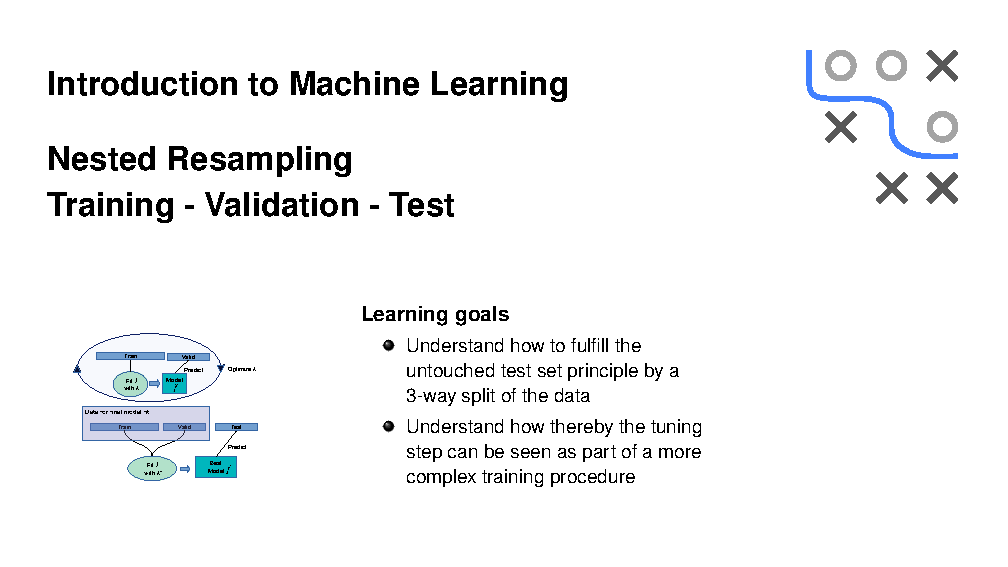
\includepdf[pages={1-last}]{slides-nested-trainvalidtest.pdf}
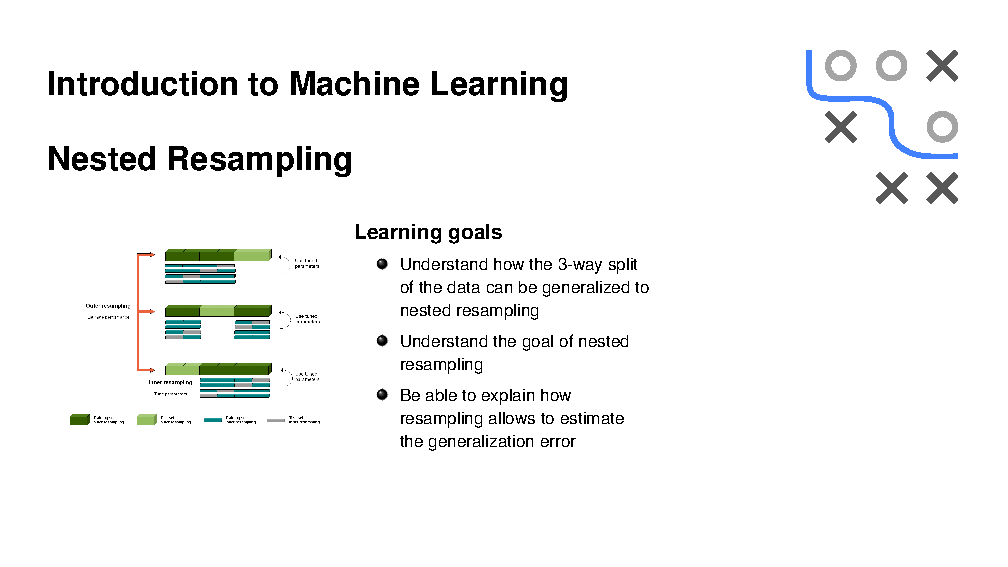
\includepdf[pages={1-last}]{slides-nested-nestedresampling.pdf}

\section{Nested Resampling with mlr3tuning}

\includepdf[pages={71-last}]{../slides/mlr3/slides-mlr3-tuning.pdf}

\section{Exercise: Nested Resampling with mlr3tuning}
\begin{frame}{Use Case Demo \& Exercise}
\begin{itemize}
\item \textbf{Demo:} \href{https://mlr3gallery.mlr-org.com/posts/2020-03-11-mlr3tuning-tutorial-german-credit/\#nested-resampling}{\underline{mlr3tuning Tutorial}} (Start at Section Nested Resampling)
\item \textbf{Exercise:} Modify the previous demo according to the following exercises.
\begin{enumerate}
\item Create an \texttt{AutoTuner} based on a random forest (\texttt{ranger}), which automatically finds the best hyperparameters for \texttt{mtry} and \texttt{replace} based on random search.
See \texttt{?ranger} for a description of the parameters and use a meaningful number of evaluations and a meaningful search space.
\item Use the \texttt{benchmark} function to compare the performance of the \texttt{AutoTuner} against an untuned \texttt{ranger} and \texttt{rpart} learner in their default hyperparameter values.
\end{enumerate}
\end{itemize}
\end{frame}

\section{ML Pipelines with mlr3pipelines}
\includepdf[pages={2-36, 67-68, 57-60, 72-last}]{../slides/mlr3/slides-mlr3-pipelines.pdf}

\section{Demo: mlr3pipelines}
\begin{frame}{Demo: mlr3pipelines}
\textbf{Demo:} \href{https://mlr3gallery.mlr-org.com/posts/2020-03-11-mlr3pipelines-tutorial-german-credit/}{\underline{mlr3pipelines Tutorial}}
\end{frame}

\section{Final Use Case}

% \section{ROC Analysis} % 30 min.
% 
\includepdf[pages={1-last}]{slides-evaluation-measures-classification-roc.pdf}
% 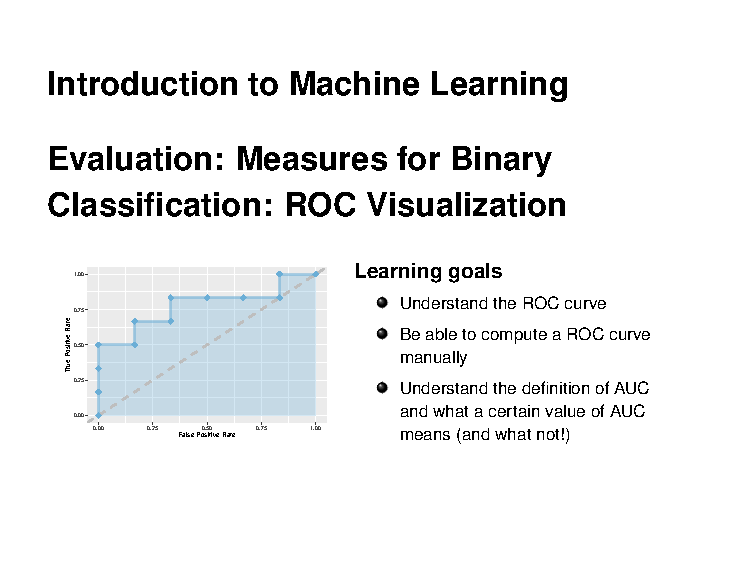
\includepdf[pages={1-16}]{slides-evaluation-measures-classification-roc-space.pdf}

\end{document}
